\documentclass[tikz,border=10pt]{standalone}
\usepackage{amsmath}
\usetikzlibrary{arrows.meta, positioning, fit}

% Define styles for different types of nodes and edges
\tikzset{
    vertex/.style={circle, draw, fill=#1!50, minimum size=1.2cm, inner sep=0},
    vertex-blue/.style={vertex=blue},
    vertex-red/.style={vertex=red},
    vertex-pink/.style={vertex=pink},
    edge-blue/.style={blue, thick, -Latex},
    edge-red/.style={red, thick, -Latex},
    dashed-edge/.style={dashed, gray, thick, -Latex},
    every label/.append style={font=\small},
}

\begin{document}
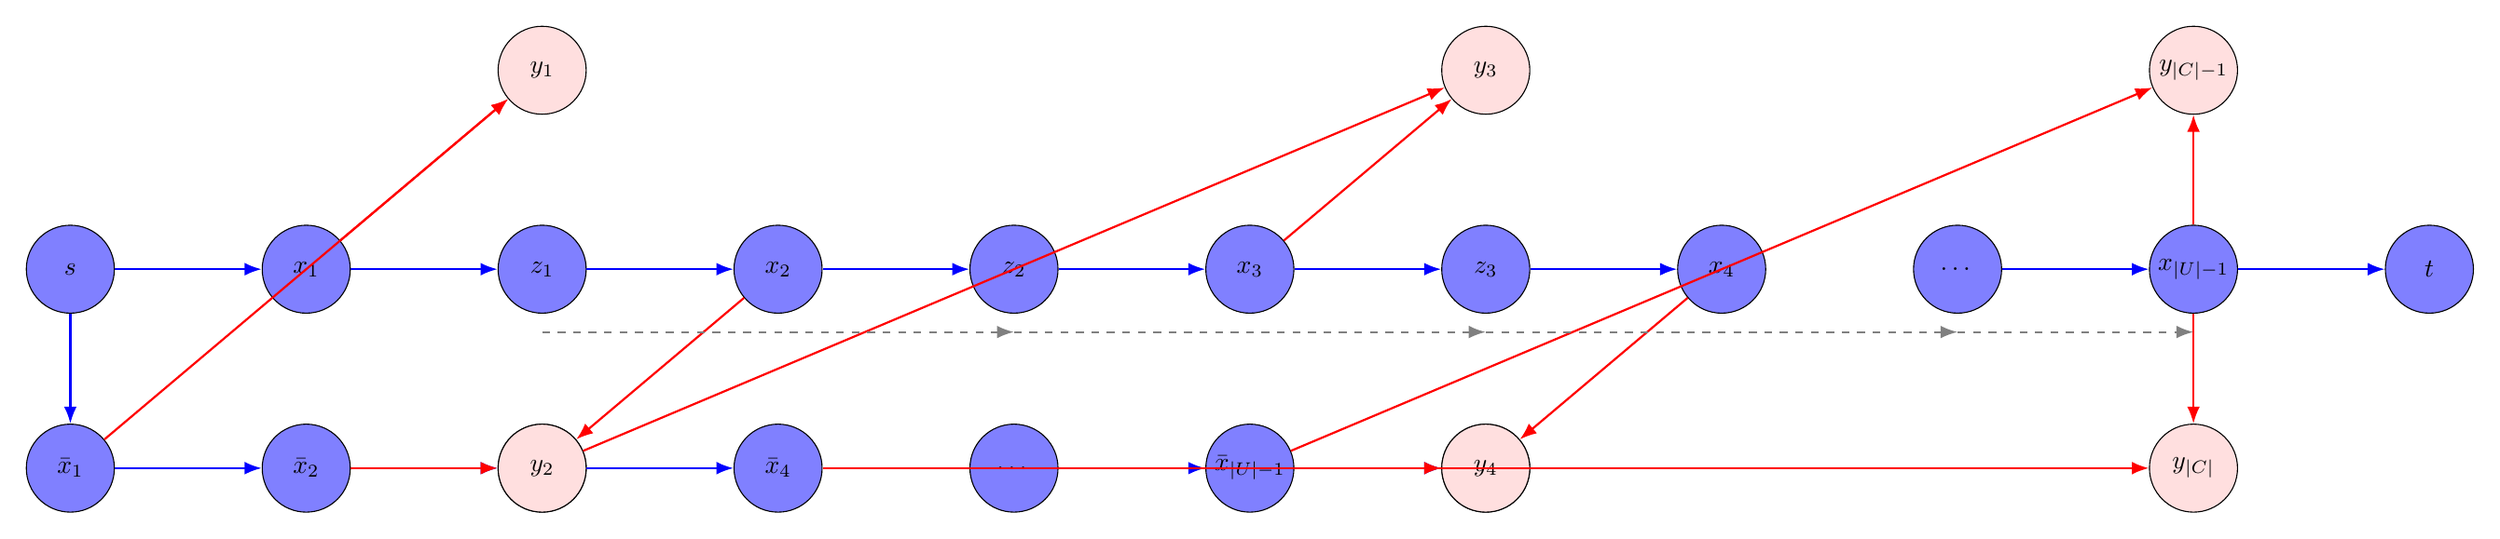
\begin{tikzpicture}[node distance=1.5cm and 2cm]

% Define nodes
\node[vertex-blue] (s) at (0,0) {$s$};
\node[vertex-blue] (x1) [right=of s] {$x_1$};
\node[vertex-blue] (z1) [right=of x1] {$z_1$};
\node[vertex-blue] (x2) [right=of z1] {$x_2$};
\node[vertex-blue] (z2) [right=of x2] {$z_2$};
\node[vertex-blue] (x3) [right=of z2] {$x_3$};
\node[vertex-blue] (z3) [right=of x3] {$z_3$};
\node[vertex-blue] (x4) [right=of z3] {$x_4$};
\node[vertex-blue] (dots1) [right=of x4] {$\dots$};
\node[vertex-blue] (xn-1) [right=of dots1] {$x_{|U|-1}$};
\node[vertex-blue] (t) [right=of xn-1] {$t$};

\node[vertex-blue] (sx1) [below=of s] {$\bar{x}_1$};
\node[vertex-blue] (sx2) [right=of sx1] {$\bar{x}_2$};
\node[vertex-blue] (sx3) [right=of sx2] {$\bar{x}_3$};
\node[vertex-blue] (sx4) [right=of sx3] {$\bar{x}_4$};
\node[vertex-blue] (dots2) [right=of sx4] {$\dots$};
\node[vertex-blue] (sxn-1) [right=of dots2] {$\bar{x}_{|U|-1}$};
\node[vertex-blue] (st) [right=of sxn-1] {$\bar{t}$};

\node[vertex-pink] (y1) [above=of z1] {$y_1$};
\node[vertex-pink] (y2) [below=of z1] {$y_2$};
\node[vertex-pink] (y3) [above=of z3] {$y_3$};
\node[vertex-pink] (y4) [below=of z3] {$y_4$};
\node[vertex-pink] (yn-1) [above=of xn-1] {$y_{|C|-1}$};
\node[vertex-pink] (yc) [below=of xn-1] {$y_{|C|}$};

% Draw blue edges (unweighted graph H)
\draw[edge-blue] (s) -- (x1);
\draw[edge-blue] (x1) -- (z1);
\draw[edge-blue] (z1) -- (x2);
\draw[edge-blue] (x2) -- (z2);
\draw[edge-blue] (z2) -- (x3);
\draw[edge-blue] (x3) -- (z3);
\draw[edge-blue] (z3) -- (x4);
\draw[edge-blue] (dots1) -- (xn-1);
\draw[edge-blue] (xn-1) -- (t);

\draw[edge-blue] (s) -- (sx1);
\draw[edge-blue] (sx1) -- (sx2);
\draw[edge-blue] (sx2) -- (sx3);
\draw[edge-blue] (sx3) -- (sx4);
\draw[edge-blue] (dots2) -- (sxn-1);
\draw[edge-blue] (sxn-1) -- (st);

% Draw red edges (additional vertices and edges with weight |U|)
\draw[edge-red] (x1) -- (y1);
\draw[edge-red] (sx1) -- (y1);
\draw[edge-red] (x2) -- (y2);
\draw[edge-red] (sx2) -- (y2);
\draw[edge-red] (x3) -- (y3);
\draw[edge-red] (sx3) -- (y3);
\draw[edge-red] (x4) -- (y4);
\draw[edge-red] (sx4) -- (y4);

\draw[edge-red] (xn-1) -- (yn-1);
\draw[edge-red] (sxn-1) -- (yn-1);
\draw[edge-red] (xn-1) -- (yc);
\draw[edge-red] (sxn-1) -- (yc);

% Add dotted lines for symmetry and alignment
\draw[dashed-edge] ([yshift=-0.25cm]z1.south) -- ([yshift=-0.25cm]z2.south);
\draw[dashed-edge] ([yshift=-0.25cm]z2.south) -- ([yshift=-0.25cm]z3.south);
\draw[dashed-edge] ([yshift=-0.25cm]z3.south) -- ([yshift=-0.25cm]dots1.south);
\draw[dashed-edge] ([yshift=-0.25cm]dots1.south) -- ([yshift=-0.25cm]xn-1.south);

\end{tikzpicture}
\end{document}